\documentclass[10pt,twocolumn]{article}
\usepackage[utf8]{inputenc}
\usepackage[T1]{fontenc}
\usepackage{lmodern}
\usepackage[margin=2cm]{geometry}
\usepackage{amsmath,amssymb}
\usepackage{graphicx}
\usepackage{booktabs}
\usepackage{array}
\usepackage[table]{xcolor}
\usepackage{caption}
\usepackage[hidelinks]{hyperref}

% Terminos en espanol sin depender de babel-spanish
\renewcommand{\abstractname}{Resumen}
\renewcommand{\figurename}{Figura}
\renewcommand{\tablename}{Tabla}
\renewcommand{\refname}{Referencias}

\captionsetup{font=small,labelfont=bf}
\setlength{\parskip}{2pt}

\title{\vspace{-1.2em}\textbf{Ciberseguridad Sostenible en el Borde: Reducci\'on de la
Huella de Carbono en la Inspecci\'on de APIs mediante C\'omputo Verde y Teor\'ia de
Juegos}}
\author{Equipo \emph{Stochastic Green Edge} (SGE)\\
\small Computaci\'on Sostenible y Ciberseguridad Cloud}
\date{\today}

\begin{document}
\maketitle

\begin{abstract}
\noindent El sector de las Tecnolog\'ias de la Informaci\'on y la Comunicaci\'on
(TIC) y, en particular, los centros de datos, representan una fracci\'on creciente del
consumo el\'ectrico mundial y de las emisiones de gases de efecto invernadero
\cite{masanet,radu}. Dentro de esta carga, la pr\'actica de seguridad dominante
---someter el $100\%$ del tr\'afico entrante de una API a inspecci\'on profunda---
impone un consumo energ\'etico elevado, constante e \emph{invariante al riesgo},
un sobreprocesamiento que contradice los principios del c\'omputo verde. Este trabajo
aborda la ciberseguridad desde la \'optica de la \textbf{sostenibilidad}: presentamos
\textbf{Stochastic Green Edge} (SGE), una defensa perimetral de dos capas ---un filtro
\emph{Edge} de baja potencia y una funci\'on \emph{Serverless} de inspecci\'on
profunda--- que activa el c\'omputo costoso \emph{solo cuando es energ\'eticamente
justificable}. La decisi\'on se optimiza como un equilibrio de Nash que iguala el
\emph{Joule marginal invertido con la seguridad marginal obtenida}. En una simulaci\'on
de $2{,}000$ peticiones, SGE reduce el consumo energ\'etico en un \textbf{$85.9\%$}
(de $30{,}010$ a $4{,}225$ Joules) y, en consecuencia, la \textbf{huella de carbono en
la misma proporci\'on}: a escala de una API de $10^{9}$ peticiones mensuales, ello
equivale a evitar del orden de \textbf{$2$ toneladas de CO\textsubscript{2} al a\~no},
manteniendo una mitigaci\'on de amenazas del $94.38\%$. Mostramos que reservar el
c\'omputo intensivo para la fracci\'on de tr\'afico realmente sospechosa es un
principio de ecodise\~no eficaz para alinear la seguridad con la descarbonizaci\'on.

\vspace{4pt}
\noindent\textbf{Palabras clave:} c\'omputo verde, huella de carbono, eficiencia
energ\'etica, computaci\'on sostenible, edge computing, serverless, equilibrio de
Nash, seguridad de APIs, inyecci\'on de prompts, AWS, ESG, B2B SaaS.
\end{abstract}

\section{Introducci\'on}
La sostenibilidad del c\'omputo se ha convertido en una preocupaci\'on de primer orden:
los centros de datos consumen ya un porcentaje significativo de la electricidad
mundial y su demanda crece con la digitalizaci\'on \cite{masanet}. El
\emph{c\'omputo verde} (\emph{green computing}) persigue reducir esa energ\'ia y las
emisiones asociadas mediante el ecodise\~no del software: eliminar el
sobreprocesamiento, aprovechar recursos de baja potencia y desplazar la carga hacia
donde la energ\'ia es m\'as limpia \cite{radu,murugesan}.

La ciberseguridad de APIs es, paradojicamente, un foco de derroche energ\'etico
oculto. La pr\'actica habitual somete \emph{cada} petici\'on a una inspecci\'on
profunda ---sanitizaci\'on exhaustiva, validaci\'on criptogr\'afica, an\'alisis de
payload--- con independencia de su riesgo real. Este gasto uniforme maximiza la
cobertura, pero desperdicia energ\'ia (y emite CO\textsubscript{2}) procesando de
forma intensiva un tr\'afico que, en su gran mayor\'ia, es leg\'itimo o trivialmente
malicioso. El problema es que la fracci\'on verdaderamente peligrosa ---ataques
dirigidos que imitan tr\'afico leg\'itimo, como la \emph{inyecci\'on de prompts}
(\emph{prompt injection}) contra APIs respaldadas por modelos de lenguaje--- \textbf{no
es directamente observable}.

\paragraph{El costo ambiental de la seguridad ``siempre al m\'aximo''.} Las defensas
tradicionales ---cortafuegos de aplicaciones web (WAF), pasarelas de API y tuber\'ias
de inspecci\'on profunda--- se aprovisionan para procesar \emph{el $100\%$ del
tr\'afico entrante a su m\'axima capacidad}: cada petici\'on atraviesa el conjunto
completo de reglas de firma, validaci\'on criptogr\'afica y, cada vez m\'as, an\'alisis
de contenido basado en aprendizaje autom\'atico o en modelos de lenguaje. Esta postura
de ``inspecci\'on total y constante'' mantiene la CPU y los aceleradores en alta
utilizaci\'on de forma permanente, con independencia de que en torno al $95\%$ del
tr\'afico sea benigno o trivialmente malicioso. El resultado es un consumo el\'ectrico
sostenido y, por la ecuaci\'on~\eqref{eq:co2}, una l\'inea base de carbono elevada y
constante ---un desperdicio energ\'etico masivo dedicado a examinar exhaustivamente
peticiones que no lo requieren. La irrupci\'on de las APIs respaldadas por modelos de
lenguaje agrava el problema: detectar una inyecci\'on de prompts puede exigir invocar
un modelo, elevando el costo energ\'etico \emph{por inspecci\'on} en varios \'ordenes
de magnitud. SGE invierte este paradigma: un filtro \emph{Edge} de baja potencia
resuelve de forma econ\'omica la mayor\'ia benigna y, guiado por el equilibrio de Nash,
\emph{solo} escala a la inspecci\'on profunda costosa la fracci\'on sospechosa,
recortando la energ\'ia ---y la huella de carbono--- de la defensa en un $85.9\%$ sin
degradar de forma apreciable la protecci\'on.

Este art\'iculo reformula la decisi\'on de ``inspeccionar o no'' como un
\textbf{problema de sostenibilidad}: minimizar la energ\'ia (y la huella de carbono)
sujeta a un nivel de seguridad aceptable. Nuestra tesis es que la inspecci\'on
profunda debe tratarse como un recurso energ\'etico escaso y asignarse
\emph{selectivamente}. Para hacerlo de forma \'optima y robusta ante un adversario
estrat\'egico, modelamos la decisi\'on como un juego no cooperativo y la resolvemos
con el equilibrio de Nash en estrategias mixtas \cite{alpcan,manshaei}, que act\'ua
como el \emph{mecanismo} para lograr el fin sostenible. Nuestras contribuciones son:
\begin{itemize}\itemsep2pt
  \item Un \textbf{modelo de sostenibilidad} de la defensa perimetral que integra un
        modelo energ\'etico por capa y un modelo de contabilidad de carbono.
  \item Una \textbf{pol\'itica de asignaci\'on energ\'etica} \'optima que reserva el
        c\'omputo intensivo para el tr\'afico de alto riesgo, derivada del equilibrio
        de Nash.
  \item Una \textbf{cuantificaci\'on de la huella de carbono} evitada, con figuras y
        estimaciones reproducibles a escala real.
\end{itemize}

\section{Estado del Arte}
\label{sec:sota}
La seguridad de aplicaciones en la nube se ha estructurado en torno a varias familias
de controles. En el per\'imetro operan los \emph{cortafuegos de aplicaciones web} (WAF)
basados en firmas y reglas gestionadas, complementados con \emph{limitaci\'on de tasa}
(\emph{rate-limiting}) y listas de reputaci\'on de IP. Frente a la denegaci\'on de
servicio se despliegan servicios de mitigaci\'on volum\'etrica y redes de distribuci\'on
de contenido. Un segundo estrato lo forman los detectores de anomal\'ias basados en
aprendizaje autom\'atico y las plataformas de gesti\'on de postura (\emph{CSPM/CNAPP}),
que buscan configuraciones err\'oneas y comportamientos an\'omalos. M\'as recientemente,
el auge de las aplicaciones respaldadas por modelos de lenguaje ha motivado
\emph{barreras de contenido} (\emph{guardrails}) espec\'ificas contra la inyecci\'on de
prompts \cite{owaspllm,owaspapi}. Paralelamente, la comunidad acad\'emica ha aplicado la
teor\'ia de juegos a la seguridad de redes, modelando la interacci\'on atacante--defensor
\cite{alpcan,manshaei}.

Pese a su madurez, el estado del arte comparte tres limitaciones estructurales. Primera,
es predominantemente \textbf{reactivo}: los controles act\'uan tras observar una firma o
una anomal\'ia, y su dise\~no optimiza la \emph{cobertura} de detecci\'on, no el
\emph{costo} de defenderse. Segunda, trata la profundidad de inspecci\'on como un
recurso \textbf{gratuito e ilimitado}: la recomendaci\'on por defecto es inspeccionar
todo el tr\'afico a m\'axima profundidad, sin un modelo expl\'icito del gasto
computacional o energ\'etico que ello implica. Tercera, y como corolario, la
\textbf{eficiencia energ\'etica y la huella de carbono de la propia defensa est\'an
ausentes} del proceso de dise\~no; los marcos de referencia industriales priorizan
riesgo y cumplimiento, pero no la sostenibilidad del mecanismo de mitigaci\'on
\cite{csa,awswaf}. Los trabajos de seguridad basados en teor\'ia de juegos, por su
parte, rara vez incorporan el costo energ\'etico como t\'ermino de la funci\'on de
utilidad. SGE se sit\'ua precisamente en esa brecha.

\subsection{Panorama de amenazas y mitigaci\'on en la nube (AWS)}
\label{sec:top10}
La Tabla~\ref{tab:top10} sintetiza diez de las clases de ataque m\'as frecuentes contra
cargas en la nube y su mitigaci\'on con servicios nativos de Amazon Web Services (AWS),
segun los marcos de referencia vigentes \cite{csa,owaspapi,owaspllm,awswaf}. La mayor\'ia
de estos controles operan bajo la premisa de inspecci\'on exhaustiva; SGE es
complementario y aporta la capa de \emph{eficiencia} de la que carecen.

\begin{table*}[t]
\centering
\small
\caption{Top 10 de ataques a la nube y su mitigaci\'on con servicios AWS. SGE act\'ua
como capa de eficiencia sobre los controles de inspecci\'on (filas destacadas).}
\label{tab:top10}
\renewcommand{\arraystretch}{1.25}
\begin{tabular}{@{}p{0.5cm} p{3.6cm} p{5.3cm} p{6.2cm}@{}}
\toprule
\textbf{\#} & \textbf{Ataque} & \textbf{Descripci\'on} & \textbf{Mitigaci\'on con servicios AWS} \\
\midrule
1 & Credenciales/IAM comprometidas & Robo o abuso de claves y roles con exceso de privilegios. & IAM (m\'inimo privilegio), IAM Access Analyzer, IAM Identity Center + MFA, GuardDuty. \\
2 & Configuraciones err\'oneas (S3 y otros) & Recursos o \emph{buckets} expuestos p\'ublicamente por error. & S3 Block Public Access, AWS Config, Security Hub, Trusted Advisor. \\
3 & Denegaci\'on de servicio (DDoS) & Saturaci\'on volum\'etrica o de capa 7 del servicio. & AWS Shield (Std/Adv), CloudFront, Route~53, reglas \emph{rate-based} de WAF. \\
\rowcolor{green!8}
4 & \textbf{Inyecci\'on (SQLi/CMDi) y \emph{prompt injection}} & Payloads maliciosos que manipulan la consulta o el modelo de lenguaje. & AWS WAF (reglas gestionadas SQLi), API Gateway (\emph{throttling}), Bedrock Guardrails, validaci\'on en Lambda. \emph{[SGE: filtrado estoc\'astico]} \\
5 & Exposici\'on/fuga de datos sensibles & Extracci\'on de datos confidenciales no cifrados. & Amazon Macie, AWS KMS (cifrado), cifrado de S3, VPC endpoints. \\
6 & Secuestro de cuenta y \emph{phishing} & Robo de sesi\'on o suplantaci\'on de identidad. & Amazon Cognito, IAM Identity Center + MFA, GuardDuty, CloudTrail. \\
7 & APIs inseguras / autenticaci\'on rota & Autorizaci\'on deficiente en endpoints expuestos. & API Gateway (\emph{authorizers}), Amazon Cognito, Verified Permissions, AWS WAF. \\
8 & Amenazas internas / abuso de privilegios & Uso indebido de accesos leg\'itimos. & CloudTrail, IAM Access Analyzer, GuardDuty, AWS Config, m\'inimo privilegio. \\
9 & Malware y \emph{cryptojacking} & Compromiso de c\'omputo para miner\'ia o persistencia. & GuardDuty (Malware Protection), Amazon Inspector, Systems Manager Patch Manager. \\
10 & SSRF y robo de metadatos & Abuso del servicio de metadatos de instancia. & IMDSv2, AWS WAF, \emph{security groups}, segmentaci\'on de VPC. \\
\bottomrule
\end{tabular}
\end{table*}

\subsection{El estado del arte aplicado a SGE}
\label{sec:sota-sge}
SGE rompe el paradigma reactivo y ``siempre al m\'aximo'' descrito arriba en tres
sentidos. \textbf{(i) De reactivo a proactivo-econ\'omico:} en lugar de decidir tras
detectar, SGE decide \emph{a priori} qu\'e peticiones merecen el gasto de detecci\'on,
tratando la inspecci\'on profunda como un recurso escaso. \textbf{(ii) Filtrado
estoc\'astico de inyecci\'on:} para el tr\'afico sospechoso ---en particular los payloads
compatibles con inyecci\'on de prompts o de c\'odigo--- SGE no aplica una regla fija y
explotable, sino una \emph{pol\'itica aleatorizada} derivada del equilibrio de Nash, que
un adversario racional no puede eludir de forma sistem\'atica. As\'i, la mayor\'ia del
tr\'afico malicioso ruidoso se neutraliza en el borde y solo la fracci\'on sigilosa
escala al motor costoso. \textbf{(iii) Descarga del servidor principal:} al resolver el
$94.65\%$ de las peticiones en la capa Edge de baja potencia, SGE reduce dr\'asticamente
la carga sobre las funciones de inspecci\'on profunda del n\'ucleo, con el consiguiente
ahorro de c\'omputo y de emisiones. En s\'intesis, SGE no sustituye a los controles de la
Tabla~\ref{tab:top10}, sino que los dota de una capa de \emph{eficiencia energ\'etica}
ausente en el estado del arte.

\section{Marco de C\'omputo Verde}
\label{sec:green}
\subsection{Modelo energ\'etico por capa}
SGE distingue dos capas de infraestructura con costos energ\'eticos radicalmente
asim\'etricos, medidos en unidades relativas de Joules/ciclos \cite{murugesan}:
\begin{equation}
\label{eq:energy}
C_{\text{edge}} = 1 \;\ll\; C_{\text{exec}} = 15 \;<\; C_{\text{cold}} = 25.
\end{equation}
El filtro \emph{Edge} es una funci\'on de baja potencia y paso r\'apido; la funci\'on
\emph{Serverless} realiza inspecci\'on profunda a un costo entre $15\times$ y
$25\times$ mayor, penalizaci\'on esta \'ultima debida al \emph{arranque en fr\'io}
(\emph{cold start}) tras un periodo de inactividad \cite{castro}. Esta relaci\'on
$1{:}15{:}25$ es el n\'ucleo del argumento verde: \emph{cada petici\'on que se
resuelve en el Edge en lugar de escalar ahorra entre $14$ y $24$ unidades de
energ\'ia}.

\subsection{Modelo de huella de carbono}
La huella de carbono de una carga de c\'omputo se contabiliza como el producto de la
energ\'ia consumida por la intensidad de carbono de la electricidad que la alimenta
\cite{masanet,radu}:
\begin{equation}
\label{eq:co2}
E_{\mathrm{CO_2}} = W \cdot \mathrm{PUE} \cdot I_{\mathrm{grid}},
\end{equation}
donde $W$ es la energ\'ia de c\'omputo (kWh), $\mathrm{PUE}$ (\emph{Power Usage
Effectiveness}) captura el sobrecosto del centro de datos ---refrigeraci\'on,
distribuci\'on--- (t\'ipicamente $1.4$--$1.6$) e $I_{\mathrm{grid}}$ es la intensidad
de carbono de la red (kgCO\textsubscript{2}eq/kWh). Como $\mathrm{PUE}$ e
$I_{\mathrm{grid}}$ son constantes para una infraestructura dada, la reducci\'on
\emph{relativa} de emisiones coincide exactamente con la reducci\'on relativa de
energ\'ia:
\begin{equation}
\label{eq:co2red}
\frac{\Delta E_{\mathrm{CO_2}}}{E_{\mathrm{CO_2}}} = \frac{\Delta W}{W}.
\end{equation}
La ecuaci\'on~\eqref{eq:co2red} es la piedra angular de este trabajo: \textbf{ahorrar
Joules es, uno a uno, ahorrar carbono}. Adem\'as, al evitar escalar al centro de
datos, el tr\'afico resuelto en el borde no incurre en el factor $\mathrm{PUE}$ ni en
la energ\'ia de transmisi\'on de red, magnitudes que~\eqref{eq:co2} amplifica sobre el
gasto bruto de c\'omputo, y puede aprovechar generaci\'on renovable local
\cite{radu}.

\section{Mecanismo de Decisi\'on Energ\'eticamente \'Optima}
\label{sec:math}
Para asignar el c\'omputo intensivo de forma \'optima y robusta, modelamos cada
petici\'on \emph{sospechosa} como una etapa de un juego no cooperativo entre un
Defensor y un Atacante \cite{alpcan}. El Defensor elige entre $D_V$ (\emph{Verde}:
permanecer en el Edge, energ\'ia m\'inima) y $D_A$ (\emph{Activa}: escalar a la
inspecci\'on Serverless). Su utilidad ante el par de acciones $(a,d)$ integra
seguridad, energ\'ia y da\~no:
\begin{equation}
\label{eq:util}
U_D(a,d) = \alpha\, R(a,d) - \beta\, C_{\text{energy}}(d) - \gamma\, C_{\text{damage}}(a,d),
\end{equation}
donde el t\'ermino $\beta\,C_{\text{energy}}$ penaliza \emph{gastar} energ\'ia y el
t\'ermino $\gamma\,C_{\text{damage}}$ penaliza \emph{no} gastarla cuando habr\'ia sido
necesario. El equilibrio resuelve esta tensi\'on.

\paragraph{El punto \'optimo energ\'etico.} Como el juego carece de equilibrio en
estrategias puras, la soluci\'on es un equilibrio mixto obtenido por el
\emph{principio de indiferencia}. La condici\'on de indiferencia del Defensor se
reduce a la igualdad
\begin{equation}
\label{eq:tradeoff}
\underbrace{\beta\,(C_{\text{serverless}}-C_{\text{edge}})}_{\text{sobrecosto energ\'etico}}
=
\underbrace{\gamma\,(1-q)\,C_{\text{damage}} + \Delta R}_{\text{da\~no evitado + detecci\'on}},
\end{equation}
cuya lectura sostenible es directa: en el equilibrio, el \textbf{Joule marginal
invertido} en inspeccionar iguala exactamente a la \textbf{seguridad marginal
obtenida}. El sistema no ``sobre-inspecciona'' ---lo que malgastar\'ia energ\'ia y
carbono sin retorno de seguridad--- ni ``sub-inspecciona''. La probabilidad de
escalado crece de forma mon\'otona con la sospecha $s\in[0,1]$ inferida por el Edge
(Figura~\ref{fig:response}), concentrando el gasto en el tr\'afico de alto riesgo.

\begin{figure}[t]
\centering
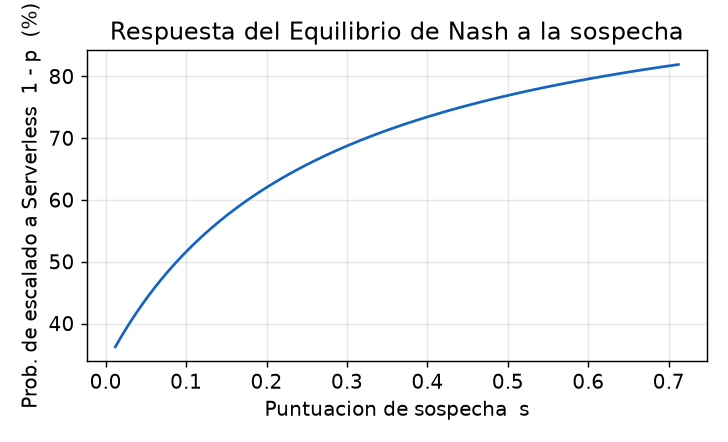
\includegraphics[width=\linewidth]{figures/fig3_response.png}
\caption{Pol\'itica energ\'etica resultante: probabilidad de activar la costosa capa
Serverless ($1-p$) frente a la sospecha $s$. El gasto es despreciable para tr\'afico
benigno y solo crece ante anomal\'ias reales.}
\label{fig:response}
\end{figure}

\section{Arquitectura Verde de Dos Capas}
\label{sec:arch}
\paragraph{Capa Edge (baja potencia).} Funci\'on de paso r\'apido con costo
$C_{\text{edge}}=1$, cercana al usuario. Extrae m\'etricas baratas y aplica
\emph{rate-limiting} que neutraliza los bots ruidosos sin invocar c\'omputo intensivo.
Ejecuta adem\'as el motor de decisi\'on de la Secci\'on~\ref{sec:math}.

\paragraph{Capa Serverless (bajo demanda).} Funci\'on ef\'imera de inspecci\'on
profunda que \emph{solo} consume recursos al invocarse, con costo $C_{\text{exec}}=15$
($C_{\text{cold}}=25$ tras inactividad \cite{castro}). Su naturaleza bajo demanda es
en s\'i misma una elecci\'on de dise\~no sostenible: a diferencia de un servicio
siempre activo, no consume energ\'ia en reposo. SGE explota esta propiedad activ\'andola
lo menos posible.

\section{Metodolog\'ia y Resultados}
\label{sec:results}
\subsection{Dise\~no experimental}
Simulamos $n=2{,}000$ peticiones (semilla $7$) con una mezcla realista: $80\%$
leg\'itimo, $15\%$ bots ruidosos y $5\%$ ataques dirigidos. Comparamos SGE
(\textbf{Adaptativo}) contra dos l\'ineas base: \textbf{Tradicional} (inspecci\'on del
$100\%$) y \textbf{Edge-only} (nunca escala). Las m\'etricas centrales son la
energ\'ia consumida y la huella de carbono derivada; la seguridad (tasa de
mitigaci\'on) act\'ua como restricci\'on de calidad de servicio. La implementaci\'on se
verific\'o con \texttt{Ruff} y $13$ pruebas en \texttt{Pytest}.

\subsection{Ahorro energ\'etico}
De las $2{,}000$ peticiones, solo $107$ ($5.35\%$) escalaron a la capa Serverless; el
$94.65\%$ restante se resolvi\'o en el Edge al costo m\'inimo. En consecuencia, el
consumo del Adaptativo se descompone en $2{,}000$ Joules del Edge m\'as $2{,}225$ de
las invocaciones profundas, totalizando $\mathbf{4{,}225}$ Joules frente a los
$\mathbf{30{,}010}$ de la inspecci\'on est\'atica: un \textbf{ahorro del $85.9\%$}
(Figura~\ref{fig:energy}). El Edge-only minimiza la energ\'ia pero deja pasar el
$100\%$ de los ataques avanzados, confirmando que la capa profunda es imprescindible
y debe usarse ---con criterio--- para la fracci\'on sigilosa.

\begin{figure}[t]
\centering
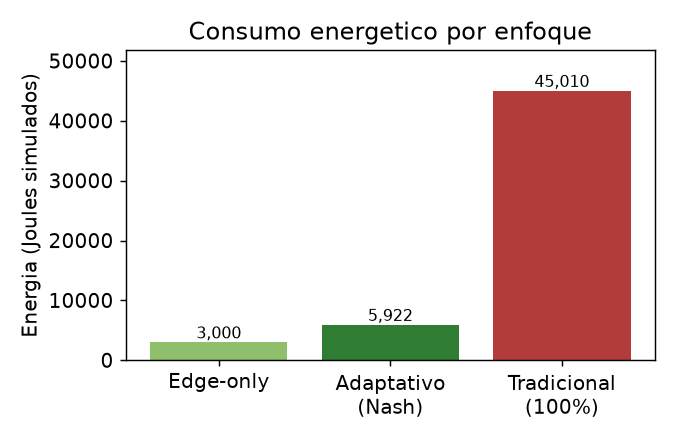
\includegraphics[width=\linewidth]{figures/fig1_energy.png}
\caption{Consumo energ\'etico por enfoque. El Adaptativo se sit\'ua cerca del piso del
Edge-only y muy por debajo de la inspecci\'on est\'atica.}
\label{fig:energy}
\end{figure}

\subsection{Reducci\'on de la huella de carbono}
Aplicando el modelo de carbono~\eqref{eq:co2}, traducimos el ahorro energ\'etico a
emisiones evitadas. Anclando de forma conservadora el costo de una inspecci\'on
profunda tibia en $e_{\text{exec}}=1$~J ($=C_{\text{exec}}=15$ unidades del modelo),
con $\mathrm{PUE}=1.5$ e $I_{\mathrm{grid}}=0.475$~kgCO\textsubscript{2}/kWh
(media mundial de la red \cite{masanet}), la Tabla~\ref{tab:carbon} y la
Figura~\ref{fig:carbon} muestran la huella anual para una API de $10^{9}$
peticiones mensuales. SGE reduce las emisiones de $2.38$ a $0.33$ toneladas de
CO\textsubscript{2} al a\~no, \textbf{evitando $\approx 2.04$ t CO\textsubscript{2}/a\~no
($85.9\%$)} ---comparable a retirar de circulaci\'on el equivalente a conducir un
autom\'ovil promedio unos $8{,}000$~km--- respecto a la inspecci\'on est\'atica.

\begin{table}[t]
\centering
\small
\caption{Huella de carbono anual por enfoque (API de $10^{9}$ pet./mes;
$\mathrm{PUE}=1.5$, $I_{\mathrm{grid}}=0.475$).}
\label{tab:carbon}
\begin{tabular}{lcc}
\toprule
\textbf{Enfoque} & \textbf{Mit.\ global} & \textbf{t CO\textsubscript{2}/a\~no} \\
\midrule
Tradicional (100\%) & $100\%$ & $2.38$ \\
\textbf{Adaptativo (Nash)} & $\mathbf{94.38}\%$ & $\mathbf{0.33}$ \\
Edge-only (0\%) & $75.53\%$ & $0.16$ \\
\bottomrule
\end{tabular}
\end{table}

\begin{figure}[t]
\centering
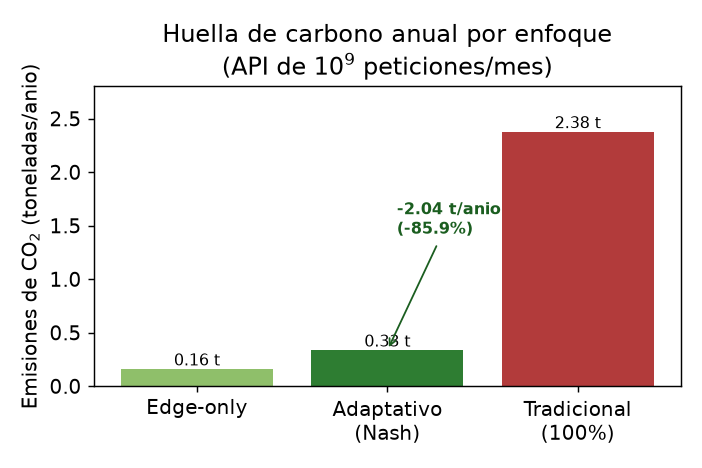
\includegraphics[width=\linewidth]{figures/fig4_carbon.png}
\caption{Huella de carbono anual por enfoque a escala de $10^{9}$ peticiones/mes. El
Adaptativo evita $\approx 2$ toneladas de CO\textsubscript{2} al a\~no frente a la
inspecci\'on est\'atica, conservando el $94.38\%$ de mitigaci\'on.}
\label{fig:carbon}
\end{figure}

Dado que el ahorro es lineal en el volumen de tr\'afico, el beneficio ambiental
escala con el tama\~no del servicio (Figura~\ref{fig:carbonscale}): para APIs de
hiperescala, las emisiones evitadas alcanzan decenas de toneladas anuales. Es
importante subrayar que, si bien las magnitudes absolutas dependen de las hip\'otesis
($e_{\text{exec}}$, $\mathrm{PUE}$, $I_{\mathrm{grid}}$), la reducci\'on
\emph{proporcional} del $85.9\%$ ---consecuencia directa de~\eqref{eq:co2red}--- es
independiente de ellas.

\begin{figure}[t]
\centering
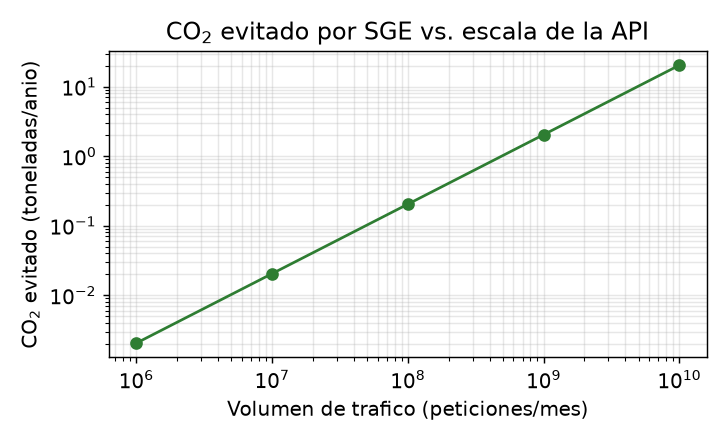
\includegraphics[width=\linewidth]{figures/fig5_carbon_scale.png}
\caption{CO\textsubscript{2} evitado por SGE frente a la escala de la API (escala
log--log). El beneficio ambiental crece linealmente con el volumen de tr\'afico.}
\label{fig:carbonscale}
\end{figure}

\subsection{La frontera sostenibilidad--seguridad}
La Figura~\ref{fig:pareto} traza la frontera entre energ\'ia y seguridad al variar el
valor asumido de la API. Permite al operador \emph{elegir su punto de compromiso
ambiental}: incluso en su configuraci\'on m\'as segura, el Adaptativo consume un orden
de magnitud menos de energ\'ia ---y por tanto de carbono--- que la inspecci\'on total.

\begin{figure}[t]
\centering
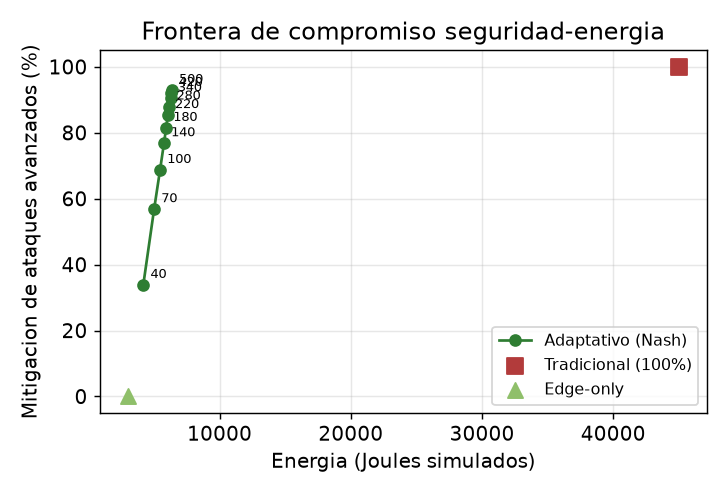
\includegraphics[width=\linewidth]{figures/fig2_pareto.png}
\caption{Frontera de compromiso sostenibilidad--seguridad. Cada punto es una
pol\'itica de equilibrio; el operador puede situarse donde prefiera sin abandonar el
r\'egimen de baja energ\'ia.}
\label{fig:pareto}
\end{figure}

\section{An\'alisis T\'ecnico y Viabilidad como \emph{Startup}}
\label{sec:viability}
\subsection{Manejo de tr\'afico masivo y carga de servidores}
El valor operativo de SGE reside en su capacidad de \emph{descarga} (\emph{offload}).
La ruta r\'apida del Edge tiene complejidad efectiva $O(1)$ por petici\'on ---extracci\'on
de m\'etricas ligeras y, a lo sumo, la resoluci\'on de un juego bimatriz $2\times2$ cuya
soluci\'on es cerrada (Secci\'on~\ref{sec:math}) y se computa en microsegundos--- de modo
que el filtro puede saturar el ancho de banda de red sin convertirse en cuello de
botella. Al resolver el $94.65\%$ del tr\'afico en esta capa, el sistema act\'ua como un
mecanismo de \emph{load shedding} inteligente: protege a las funciones de inspecci\'on
profunda del n\'ucleo de los picos de tr\'afico y de los ataques de agotamiento de
recursos, estabilizando la latencia de cola (\emph{tail latency}) y permitiendo un
escalado horizontal m\'as econ\'omico. En una arquitectura cloud t\'ipica, la capa Edge se
materializa como \emph{middleware} sin estado replicable (p.\,ej.\ un filtro en la
pasarela de API o una funci\'on de borde), mientras que el motor de inspecci\'on ---y su
costo--- se invoca bajo demanda.

\subsection{Elecci\'on de lenguajes de programaci\'on}
La naturaleza de dos capas sugiere una arquitectura \emph{poligl\'ota} alineada con las
pr\'acticas cloud-native. Para la \textbf{pasarela/Edge} recomendamos \textbf{Go}: su
modelo de concurrencia basado en \emph{goroutines}, su recolector de basura de baja
latencia, su compilaci\'on a un binario est\'atico y su reducido consumo de memoria lo
hacen id\'oneo para servicios de red de alto rendimiento ---es el lenguaje de sistemas
cloud de referencia (Kubernetes, Envoy, Traefik, Cloudflare). Para el \textbf{motor
matem\'atico} recomendamos \textbf{Python}: su ecosistema cient\'ifico (NumPy,
SciPy) permite expresar y calibrar el modelo de Nash con rapidez, y es el estilo del
prototipo actual. La comunicaci\'on entre capas puede resolverse v\'ia \texttt{gRPC} o,
dado que el equilibrio $2\times2$ es de forma cerrada, reimplementando la ruta caliente
directamente en Go y reservando Python para la calibraci\'on \emph{offline} de
par\'ametros y la experimentaci\'on. Esta separaci\'on ---Go para el plano de datos,
Python para el plano de an\'alisis--- maximiza tanto el rendimiento como la velocidad de
iteraci\'on.

\subsection{Viabilidad como modelo de negocio (B2B SaaS)}
SGE es adaptable a un producto \emph{B2B SaaS} con una propuesta de valor doble y poco
habitual en el mercado de seguridad. \textbf{(1) Reducci\'on de costos de
infraestructura:} al recortar hasta un $\sim\!86\%$ el c\'omputo de inspecci\'on, el
cliente reduce directamente su factura de CPU/serverless, un argumento comercial
inmediato y medible. \textbf{(2) Cumplimiento ambiental (ESG):} la reducci\'on de la
huella de carbono es \emph{cuantificable y auditable} (Secci\'on~\ref{sec:results}),
lo que la convierte en una palanca concreta para los reportes de sostenibilidad ---en
alcance~2 y~3--- exigidos por marcos regulatorios crecientes y por metodolog\'ias como
la Software Carbon Intensity \cite{gsf}. La entrega puede realizarse como \emph{plugin}
de pasarela o funci\'on de borde (p.\,ej.\ compatible con entornos serverless o de
\emph{edge}), minimizando la fricci\'on de integraci\'on, con un modelo de tarificaci\'on
por mill\'on de peticiones o por ahorro compartido. El p\'ublico objetivo natural son las
empresas ``API-first'' y, de forma destacada, los proveedores de aplicaciones basadas
en modelos de lenguaje, para quienes la inyecci\'on de prompts es una amenaza emergente y
el costo por inspecci\'on es especialmente alto. \textbf{Conclusi\'on de viabilidad:}
SGE combina un ahorro de costos tangible con una ventaja de cumplimiento ESG y una
defensa t\'ecnica diferenciada (la pol\'itica estoc\'astica \'optima), lo que lo hace
viable como \emph{startup}; los principales riesgos a validar son la precisi\'on de
detecci\'on en tr\'afico real y la facilidad de integraci\'on en las arquitecturas de los
clientes.

\section{Discusi\'on}
\label{sec:discussion}
Los resultados muestran que la teor\'ia de juegos es una herramienta eficaz de
\emph{ecodise\~no}: permite capturar la mayor parte del valor de seguridad de la
inspecci\'on exhaustiva con una fracci\'on de su energ\'ia y, por~\eqref{eq:co2red}, de
su huella de carbono. El enfoque es sin\'ergico con otras estrategias verdes: al
concentrar el $94.65\%$ de las peticiones en el borde de baja potencia, habilita el
aprovechamiento de energ\'ia renovable local y reduce la dependencia de centros de
datos con alto $\mathrm{PUE}$ \cite{radu,masanet}.

\paragraph{Limitaciones.} (i) Los costos energ\'eticos son unidades relativas
simuladas; una calibraci\'on con mediciones f\'isicas de potencia refinar\'ia las
estimaciones absolutas de carbono \cite{murugesan}. (ii) $\mathrm{PUE}$ e
$I_{\mathrm{grid}}$ var\'ian por regi\'on y hora; una pol\'itica \emph{consciente del
carbono} (\emph{carbon-aware}) podr\'ia escalar preferentemente cuando la red es m\'as
limpia. (iii) La detecci\'on Serverless se idealiza como perfecta. (iv) Cada petici\'on
es una etapa independiente; un juego multi-etapa con estado permitir\'ia pol\'iticas
con memoria \cite{alpcan}.

\section{Conclusiones}
\label{sec:conclusion}
Presentamos SGE desde la perspectiva de la sostenibilidad: una defensa perimetral que
trata la inspecci\'on profunda como un recurso energ\'etico escaso y lo asigna mediante
el equilibrio de Nash, igualando el Joule invertido con la seguridad obtenida. El
resultado es un ahorro energ\'etico del $85.9\%$ y una reducci\'on proporcional de la
huella de carbono ---del orden de $2$ toneladas de CO\textsubscript{2} anuales a escala
de $10^{9}$ peticiones/mes--- conservando un $94.38\%$ de mitigaci\'on de amenazas.
SGE demuestra que la ciberseguridad y la descarbonizaci\'on no son objetivos opuestos:
con el mecanismo de asignaci\'on adecuado, reforzar una refuerza la otra. Como trabajo
futuro proponemos pol\'iticas \emph{carbon-aware} que incorporen la intensidad de
carbono en tiempo real y la medici\'on f\'isica del consumo por capa.

\begin{thebibliography}{9}
\small
\bibitem{masanet} E.~Masanet, A.~Shehabi, N.~Lei, S.~Smith, and J.~Koomey.
\emph{Recalibrating global data center energy-use estimates}. Science,
367(6481):984--986, 2020.
\bibitem{radu} L.~D.~Radu. \emph{Green Cloud Computing: An Energy-Efficient
Ecodesign for IT}. Energies, 2017.
\bibitem{murugesan} S.~Murugesan and G.~R.~Gangadharan (eds.). \emph{Harnessing Green
IT: Principles and Practices}. Wiley, 2012.
\bibitem{castro} P.~Castro, V.~Ishakian, V.~Muthusamy, and A.~Slominski. \emph{The
rise of serverless computing}. Communications of the ACM, 62(12):44--54, 2019.
\bibitem{alpcan} T.~Alpcan and T.~Ba\c{s}ar. \emph{Network Security: A Decision and
Game-Theoretic Approach}. Cambridge University Press, 2010.
\bibitem{manshaei} M.~H.~Manshaei, Q.~Zhu, T.~Alpcan, T.~Ba\c{s}ar, and J.-P.
Hubaux. \emph{Game theory meets network security and privacy}. ACM Computing Surveys
(CSUR), 45(3):1--39, 2013.
\bibitem{owaspllm} OWASP Foundation. \emph{OWASP Top 10 for Large Language Model
Applications}. 2023--2025.
\bibitem{owaspapi} OWASP Foundation. \emph{OWASP API Security Top 10}. 2023.
\bibitem{csa} Cloud Security Alliance. \emph{Top Threats to Cloud Computing: The
Pandemic Eleven}. 2022.
\bibitem{awswaf} Amazon Web Services. \emph{AWS Well-Architected Framework: Security
Pillar}. 2023.
\bibitem{gsf} Green Software Foundation. \emph{Software Carbon Intensity (SCI)
Specification}. 2024.
\end{thebibliography}

\end{document}
